\chapter{System Design and Realisation}


\section*{Introduction}
In this chapter, we focus on the technical realization of BViral Control Center. We present the system architecture, justify our technology choices, describe the development environment and tools, and showcase the implemented interfaces through screenshots.

% ══════════════════════════════════════════════════════════════
\section{System Architecture}
% ══════════════════════════════════════════════════════════════
This section describes the overall system architecture of the BViral Control Center platform. It presents the structural organization of the system, highlighting how the different components are distributed across the monorepo workspace, how they interact within a client-server model, and how the backend is structured following an MVC-inspired pattern. This architectural design ensures modularity, scalability, and clear separation of concerns across all system layers.
\subsection{Monorepo Workspace Architecture}

BViral Control Center is organized as a \textbf{pnpm monorepo workspace}, a modern approach that allows multiple packages (frontend, backend, shared libraries) to coexist in a single repository while maintaining clear separation of concerns.

% \begin{figure}[H]
%     \centering
%     \includegraphics[width=0.85\textwidth]{figures/arch_monorepo.png}
%     \caption{pnpm Monorepo workspace architecture}
%     \label{fig:arch-monorepo}
% \end{figure}

The workspace is divided into three layers:

\begin{itemize}
    \item \textbf{artifacts/} --- Deployable applications:
    \begin{itemize}
        \item \texttt{bviral-dashboard}: React/Vite frontend dashboard
        \item \texttt{api-server}: Fastify REST API backend
        \item \texttt{openvideo}: Vendored BVIRAL Video Editor (Next.js)
        \item \texttt{mockup-sandbox}: UI prototyping sandbox
    \end{itemize}
    \item \textbf{lib/} --- Shared packages:
    \begin{itemize}
        \item \texttt{db}: Drizzle ORM schema and database helpers
        \item \texttt{api-spec}: OpenAPI specification and codegen config
        \item \texttt{api-zod}: Generated Zod validation schemas
        \item \texttt{api-client-react}: Generated React API client
    \end{itemize}
    \item \textbf{scripts/} --- Utility and automation scripts
\end{itemize}

\subsection{Client-Server Architecture}

The system follows a classic \textbf{client-server architecture} with clear separation between the presentation layer and the business/data layers.

% \begin{figure}[H]
%     \centering
%     \includegraphics[width=0.9\textwidth]{figures/arch_client_server.png}
%     \caption{Client-Server architecture of BViral}
%     \label{fig:arch-cs}
% \end{figure}

\begin{itemize}
    \item \textbf{Presentation Tier (Client):} The React/Vite dashboard served at \texttt{localhost:5173}. It communicates with the API via RESTful HTTP requests and renders the UI using React components, Tailwind CSS, and Framer Motion.
    \item \textbf{Business Logic Tier (API Server):} The Fastify server at \texttt{localhost:3001} handles authentication, OAuth flows, CRUD operations, and orchestrates the BullMQ post-publishing worker.
    \item \textbf{Data Tier:} PostgreSQL database (hosted via Supabase) managed through Drizzle ORM with type-safe schemas and Row Level Security (RLS) policies. Redis is used for BullMQ job queues.
    \item \textbf{AI Processing Tier:} Python-based AI video enhancement pipeline using PyTorch, Real-ESRGAN, GFPGAN, and OpenCV, running independently or integrated via API calls.
\end{itemize}

\subsection{MVC-Inspired Pattern}

The API server follows an MVC-inspired layered architecture:

\begin{itemize}
    \item \textbf{Routes (Controller):} Define HTTP endpoints, handle request validation, and delegate to services. Organized under \texttt{/api/v1/} with sub-routers for accounts, posts, videos, analytics, alerts, and users.
    \item \textbf{Services (Business Logic):} Contain the core business logic for each domain. Services include \texttt{accounts.service}, \texttt{posts.service}, \texttt{analytics.service}, \texttt{youtube.service}, \texttt{tiktok.service}, \texttt{meta.service}, \texttt{videos.service}, \texttt{alerts.service}, and \texttt{platform-publisher.service}.
    \item \textbf{Schema/Repository (Model):} Drizzle ORM schemas define the database structure. Repositories provide data access methods with type-safe queries.
\end{itemize}

\subsection{Fastify Plugin Architecture}

The API server is built on top of Fastify's plugin system. Plugins are auto-loaded from \texttt{src/plugins/} in a strict, numbered order so that each plugin can safely depend on the ones registered before it:

\begin{itemize}
    \item \texttt{00-config} --- environment loading and configuration parsing.
    \item \texttt{10-observability} --- structured request/response logging with request-id correlation.
    \item \texttt{20-cors} --- CORS allow-list from \texttt{CORS\_ORIGINS}.
    \item \texttt{25-multipart} --- multipart parser for video uploads.
    \item \texttt{30-database} --- PostgreSQL connection pool (configurable \texttt{dbPoolMax}) and the Drizzle instance.
    \item \texttt{35-storage} --- Supabase service-role client for privileged storage operations.
    \item \texttt{38-queues} --- BullMQ queue accessors (post-publishing, video-processing, analytics-refresh, ai-processing) and the \texttt{queuesAdmin} decorator used by the System Health page.
    \item \texttt{40-repositories} --- dependency-injected repositories (accounts, posts, videos, analytics, alerts, users, admin-posts, admin-videos, admin-audit).
    \item \texttt{45-ai} --- AI processing pipeline wiring (LTX, captioning, enhancement).
    \item \texttt{50-auth} --- Supabase JWT verification, role resolution, suspension check, and the \texttt{authenticate} / \texttt{requireRole} decorators.
\end{itemize}

Every domain route (\texttt{/api/v1/posts}, \texttt{/api/v1/accounts}, \texttt{/api/v1/admin/*}, \ldots) is itself loaded by \texttt{@fastify/autoload}, which keeps the route tree mechanically consistent with the directory layout.

% ══════════════════════════════════════════════════════════════
\section{Technology Choices}
% ══════════════════════════════════════════════════════════════
This section presents the main technologies used in the development of the BViral Control Center platform. The chosen stack was selected to ensure high performance, scalability, and maintainability across both frontend and backend layers, while also supporting real-time processing, AI integration, and efficient data management. Each technology plays a specific role within the system architecture, contributing to the overall functionality of the application.
\subsection{React \& Vite (Frontend)}

 \begin{figure}[H]
     \centering
     
\includegraphics[width=0.25\textwidth]{logos/react.png}
     \caption{React Frontend Framework}
     \label{fig:react}
 \end{figure}

  \begin{figure}[H]
     \centering
     
\includegraphics[width=0.25\textwidth]{logos/vite.png}
     \caption{Vite}
     \label{fig:react}
 \end{figure}

React 19 is a declarative, component-based JavaScript library for building user interfaces, maintained by Meta. Combined with Vite 7, a next-generation build tool, it provides near-instant hot module replacement (HMR) during development and optimized production builds. Key frontend libraries include:

\begin{itemize}
    \item \textbf{Tailwind CSS 4:} utility-first CSS framework for rapid, consistent styling.
    \item \textbf{Framer Motion:} production-ready animation library for React.
    \item \textbf{Wouter:} lightweight client-side router.
    \item \textbf{TanStack React Query:} data fetching and server-state management.
    \item \textbf{Lucide React:} modern, customizable icon library.
    \item \textbf{Recharts:} composable charting library for analytics visualization.
\end{itemize}

\subsection{Fastify (Backend)}

Fastify is a high-performance, low-overhead Node.js web framework. It is designed for speed and developer experience, featuring:

\begin{itemize}
    \item Schema-based request/response validation with AJV.
    \item Plugin-based architecture with auto-loading.
    \item Built-in logging via Pino with production-grade redaction.
    \item Native TypeScript support.
\end{itemize}

\begin{figure}[H]
    \centering
    
\includegraphics[width=0.25\textwidth]{logos/fastify.png}
    \caption{Fastify backend framework}
    \label{fig:fastify-logo}
\end{figure}

\subsection{PostgreSQL \& Drizzle ORM (Database)}

PostgreSQL is a powerful, open-source relational database system. We use Supabase as a hosted PostgreSQL provider, which adds built-in authentication and Row Level Security.

Drizzle ORM provides a type-safe, SQL-like query builder for TypeScript with:

\begin{itemize}
    \item Schema-as-code with full TypeScript type inference.
    \item Built-in Supabase RLS policy support.
    \item Zero-dependency, lightweight runtime.
    \item Push-based migration for schema changes.
\end{itemize}

\begin{figure}[H]
    \centering
    
\includegraphics[width=0.35\textwidth]{logos/postgre.png}
    \caption{Database PostgreSQL}
    \label{fig:PostgreSQL}
\end{figure}

\begin{figure}[H]
    \centering
    
\includegraphics[width=0.35\textwidth]{logos/supabase.png}
    \caption{Supabase database platform}
    \label{fig:supabase-logo}
\end{figure}

\begin{figure}[H]
    \centering
    
\includegraphics[width=0.35\textwidth]{drizzle.png}
    \caption{Drizzle ORM}
    \label{fig:drizzle-logo}
\end{figure}

\subsection{Redis \& BullMQ (Job Queue)}

Redis is used as the backing store for BullMQ, a robust Node.js job queue for managing scheduled post publishing. The worker restores pending jobs on restart and processes posts at their scheduled time, calling the appropriate platform API.

\begin{figure}[H]
    \centering
    
\includegraphics[width=0.3\textwidth]{logos/redis.png}
    \caption{Redis}
    \label{fig:Redis}
\end{figure}

\subsection{PyTorch, Real-ESRGAN \& GFPGAN (AI Pipeline)}

The AI video enhancement pipeline leverages:

\begin{itemize}
    \item \textbf{PyTorch:} deep learning framework with GPU and parallel CPU support.
    \item \textbf{Real-ESRGAN:} state-of-the-art super-resolution model for upscaling video frames (2x or 4x).
    \item \textbf{GFPGAN:} face restoration model that enhances facial details in video frames.
    \item \textbf{OpenCV:} computer vision library for classical filter processing (bilateral, Gaussian, median, unsharp mask).
    \item \textbf{FFmpeg:} multimedia framework for frame extraction, audio handling, and video encoding (H.264/H.265/AV1).
\end{itemize}

\begin{figure}[H]
    \centering
    
\includegraphics[width=0.35\textwidth]{logos/pytorch.png}
    \caption{Pytorch}
    \label{fig:Pytorch}
\end{figure}

\subsection{TypeScript (Language)}

TypeScript is used across the entire stack (frontend, backend, and shared libraries), providing:

\begin{itemize}
    \item Static type checking at compile time.
    \item Enhanced IDE support with autocompletion and refactoring.
    \item Shared type definitions between frontend and backend via the monorepo.
    \item Zod schema validation for runtime type safety.
\end{itemize}

\begin{figure}[H]
    \centering
    
\includegraphics[width=0.25\textwidth]{logos/typescript.png}
    \caption{Typescript}
    \label{fig:Typescript}
\end{figure}

% ══════════════════════════════════════════════════════════════
\section{Development Environment and Tools}
% ══════════════════════════════════════════════════════════════

\begin{table}[H]
\centering
\caption{Development tools used in the project}
\label{tab:tools}
\begin{tabularx}{\textwidth}{|l|X|}
\hline
\textbf{Tool} & \textbf{Purpose} \\
\hline
Visual Studio Code & Primary code editor with TypeScript, ESLint, and Prettier extensions \\
\hline
Node.js 24 & JavaScript runtime for the API server and build tools \\
\hline
pnpm & Fast, disk-efficient package manager with workspace support \\
\hline
Git / GitHub & Version control and collaborative development \\
\hline
Postman & API testing and endpoint documentation \\
\hline
Supabase Studio & Database management, RLS policy testing, and SQL queries \\
\hline
Google Colab & GPU-accelerated environment for AI pipeline development \\
\hline
StarUML & UML diagram creation for conceptual design \\
\hline
ngrok & HTTPS tunneling for TikTok OAuth local development \\
\hline
\end{tabularx}
\end{table}

% ══════════════════════════════════════════════════════════════
\section{Interfaces}
% ══════════════════════════════════════════════════════════════
This section presents the main user interfaces of the BViral Control Center platform. It illustrates the different screens available to content creators and administrators, highlighting how each module is translated into an intuitive and interactive graphical interface. These interfaces are designed to ensure usability, accessibility, and efficient interaction with the system’s core functionalities.
\subsection{Dashboard (Home)}

The main dashboard provides an at-a-glance overview of the creator's social media performance. It displays key performance indicators (KPIs) including total views, engagement rate, total followers, and revenue. Interactive charts show performance trends over time, and a recent activity feed highlights the latest posts and alerts.

\begin{figure}[H]
    \centering
    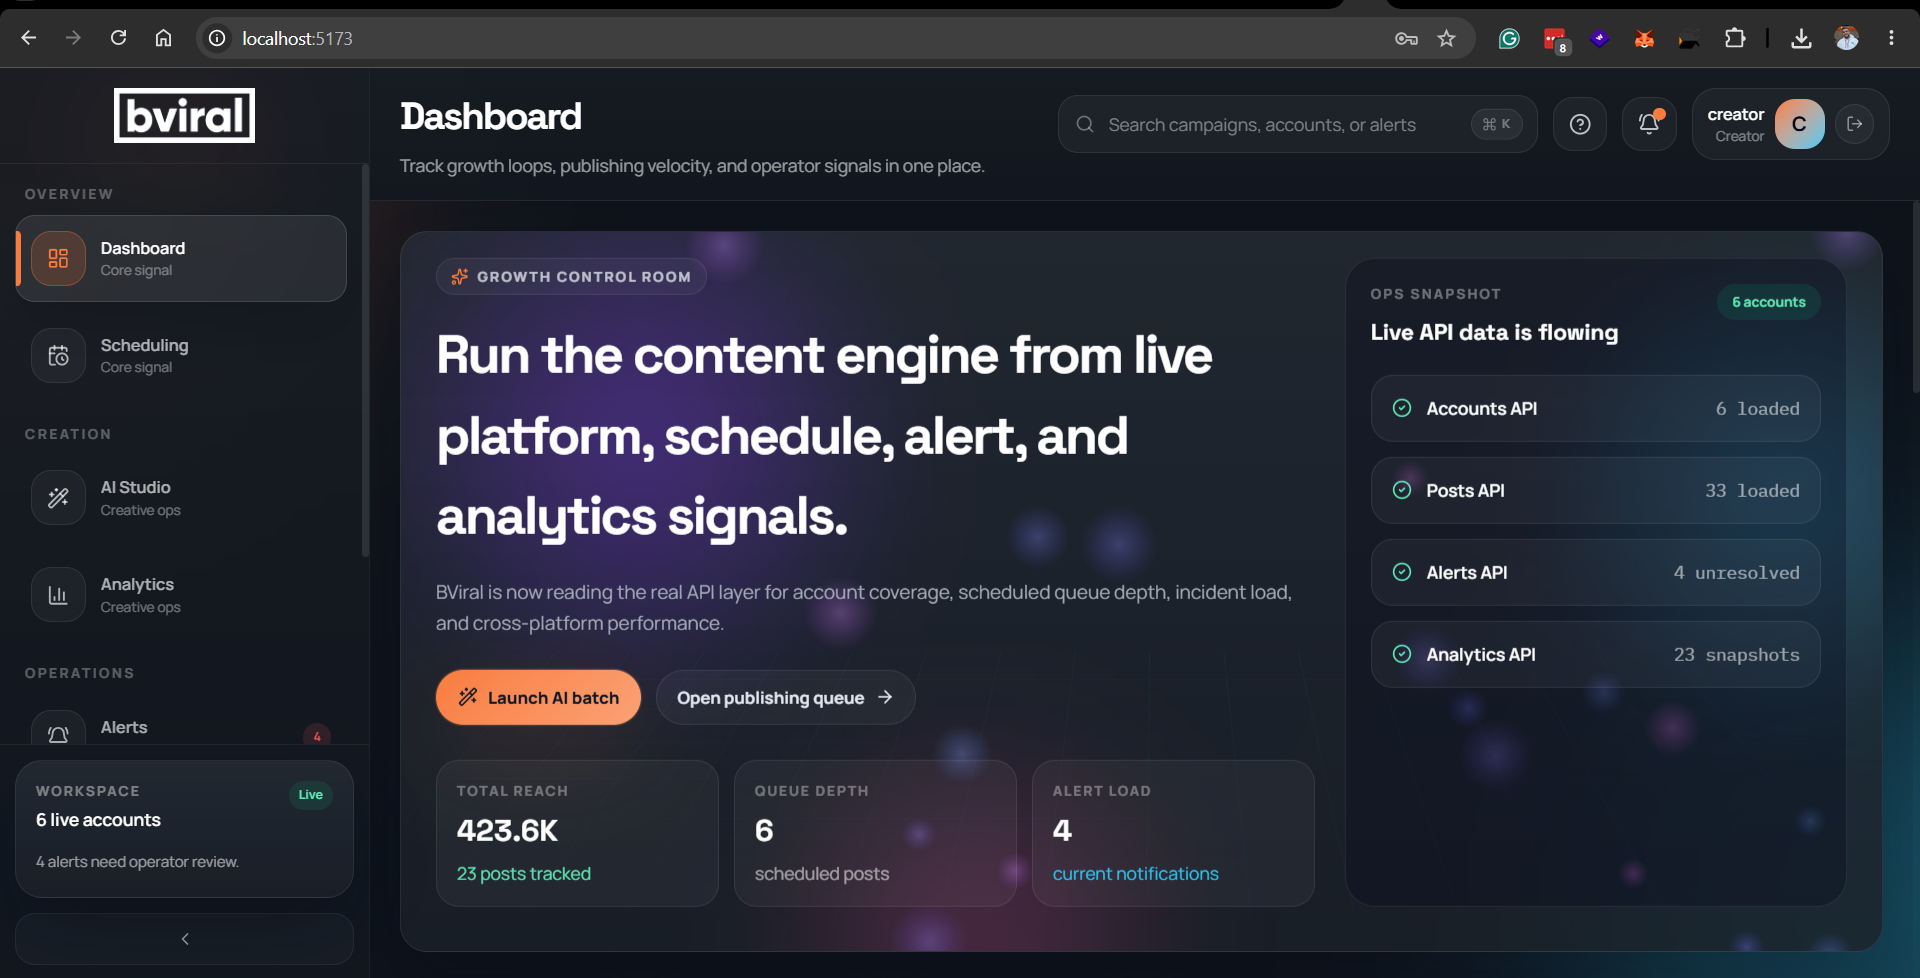
\includegraphics[width=\textwidth]{screens/Home.png}
    \caption{Interface: Dashboard overview}
    \label{fig:ui-dashboard}
\end{figure}

\subsection{Video Scheduling}

The scheduling page presents a visual calendar interface where creators can view, create, and manage scheduled posts. A side panel allows creating new posts by selecting a video, target platform, connected account, and schedule time. Posts are color-coded by status: blue for scheduled, green for posted, and red for failed.

\begin{figure}[H]
    \centering
    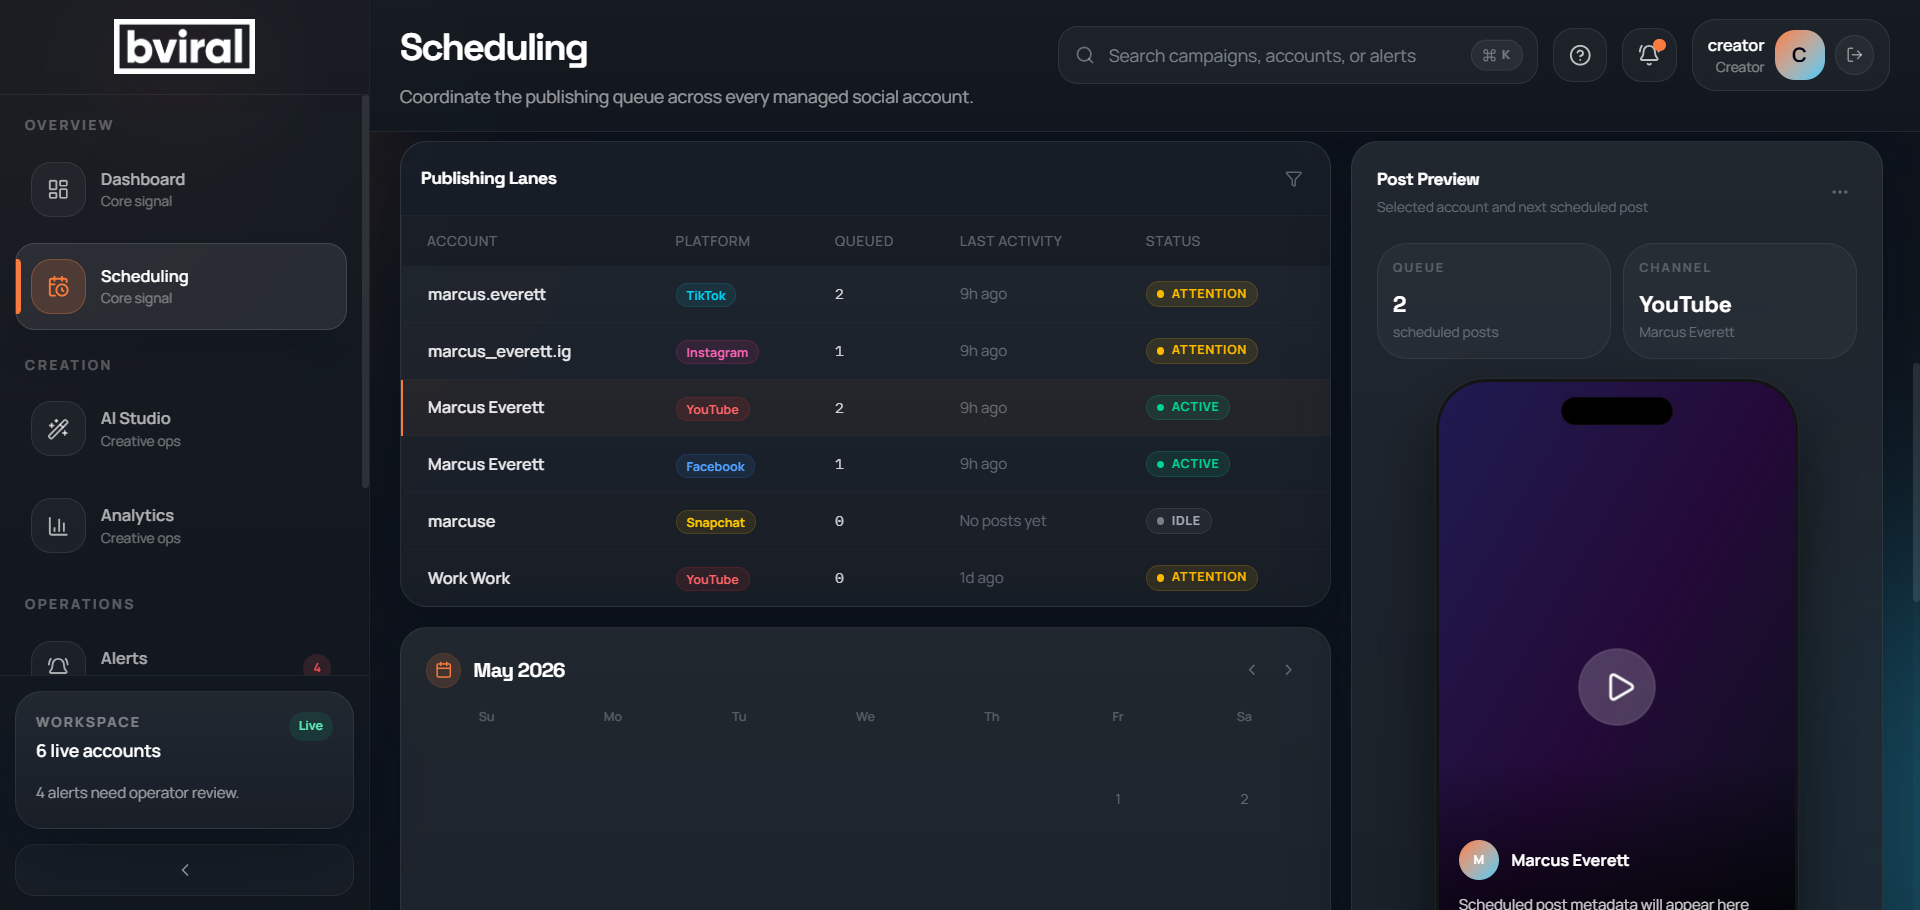
\includegraphics[width=\textwidth]{screens/scheduling.png}
    \caption{Interface: Video scheduling calendar}
    \label{fig:ui-scheduling}
\end{figure}

\subsection{Account Management}

The accounts page displays all connected social media accounts organized by platform. Each account card shows the platform icon, account name, and connection status. ``Connect'' buttons initiate the OAuth flow for each supported platform (YouTube, TikTok, Meta).

\begin{figure}[H]
    \centering
    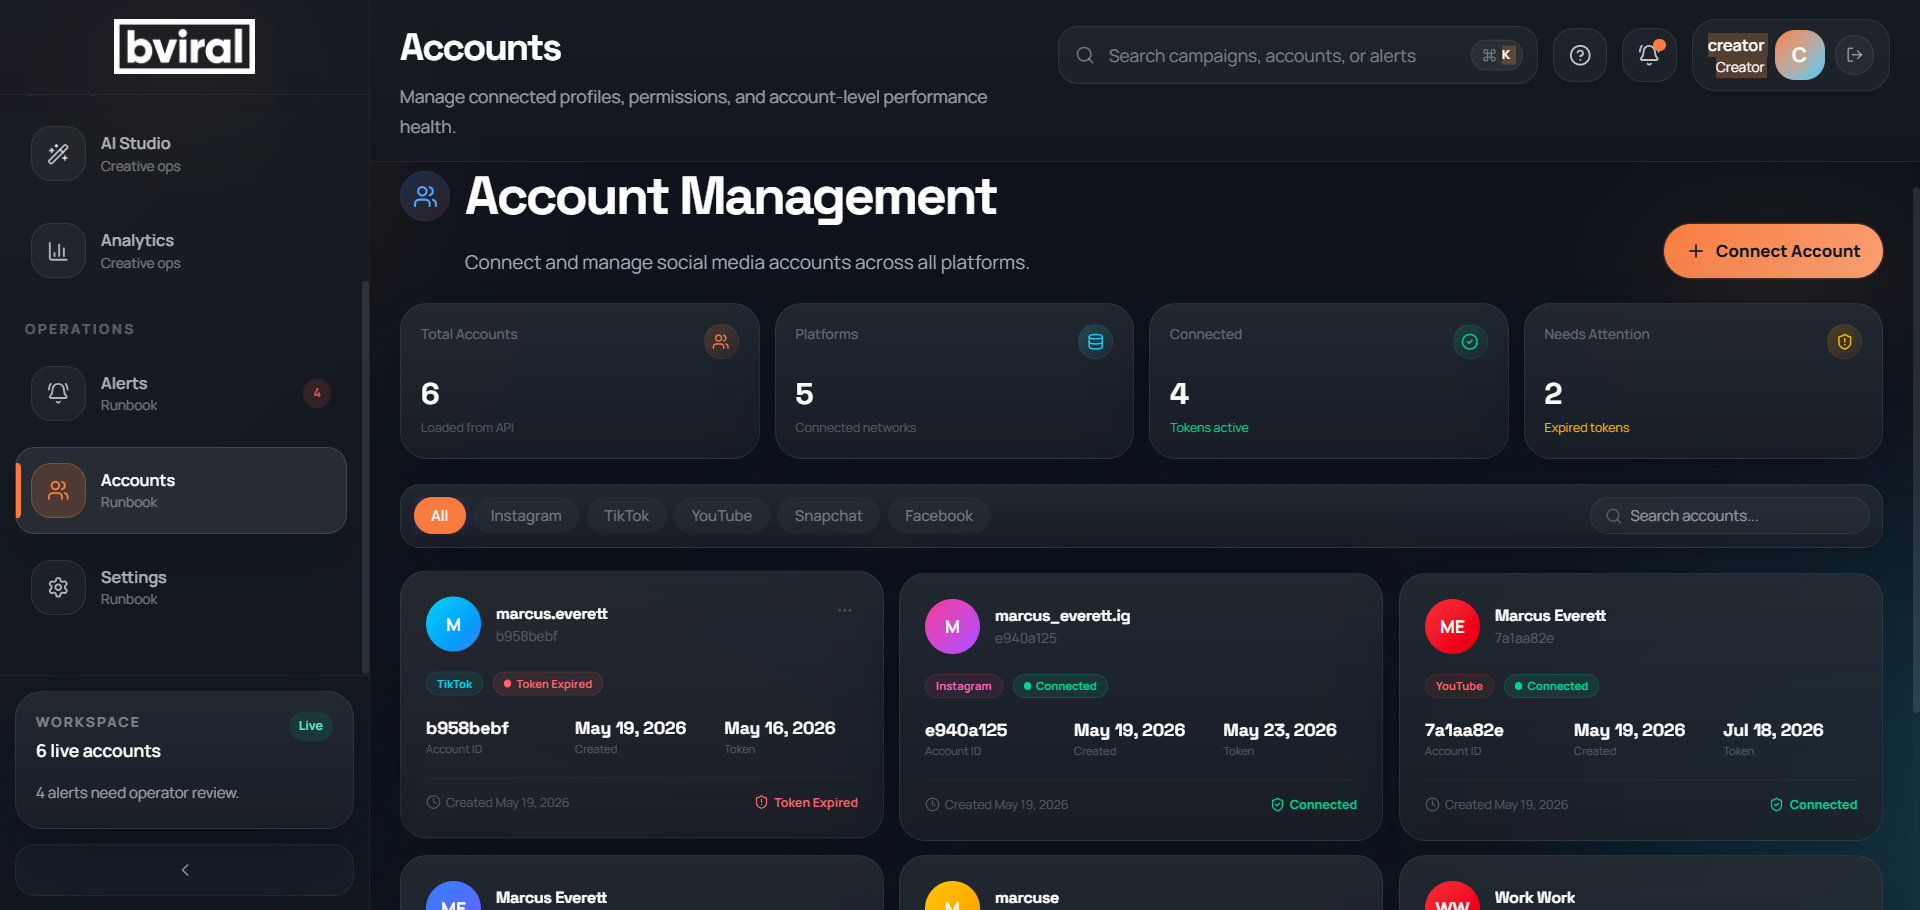
\includegraphics[width=\textwidth]{screens/accounts.png}
    \caption{Interface: Account management}
    \label{fig:ui-accounts}
\end{figure}

\subsection{Analytics Dashboard}

The analytics page provides comprehensive performance monitoring with interactive charts and filters. Users can view aggregated metrics (views, likes, comments, shares, revenue), filter by platform and time period, and visualize engagement trends through line charts, bar charts, and pie charts.

\begin{figure}[H]
    \centering
    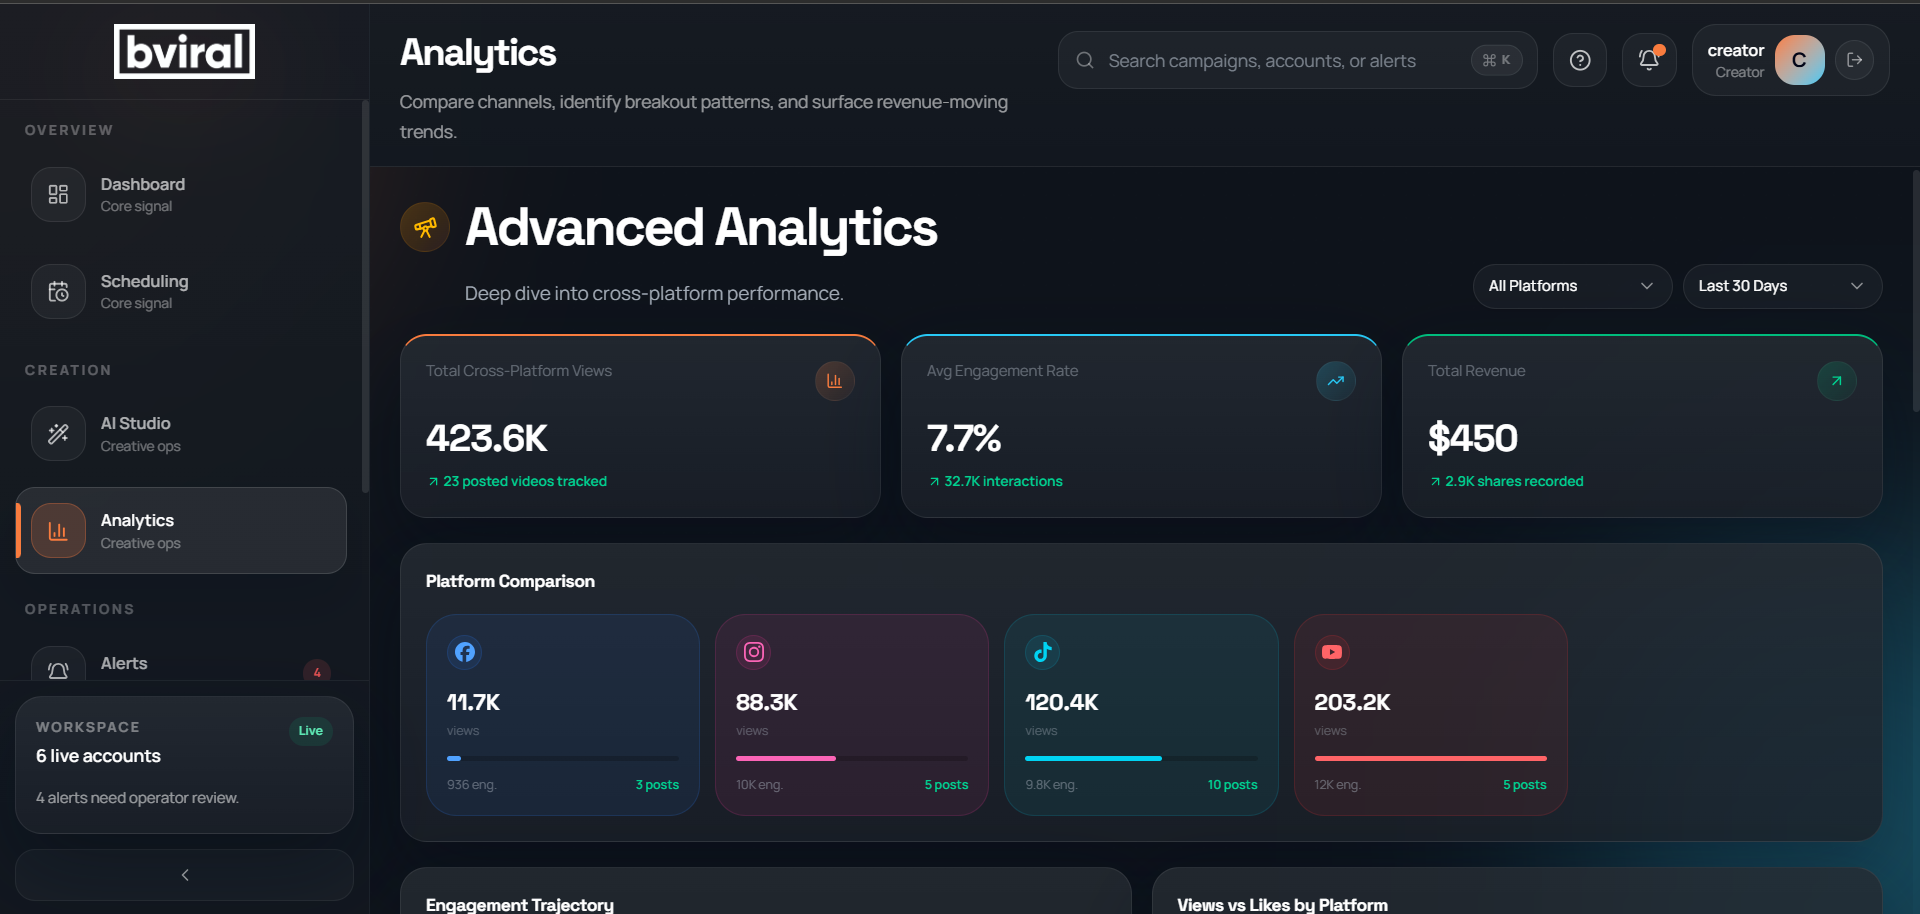
\includegraphics[width=\textwidth]{screens/analytics.png}
    \caption{Interface: Analytics dashboard}
    \label{fig:ui-analytics}
\end{figure}

\subsection{AI Video Studio}

The AI Video Studio provides access to the video enhancement pipeline and the integrated BVIRAL Video Editor. Users can upload videos, configure enhancement parameters (mode, filters, resolution), and preview results with quality metrics.

\begin{figure}[H]
    \centering
    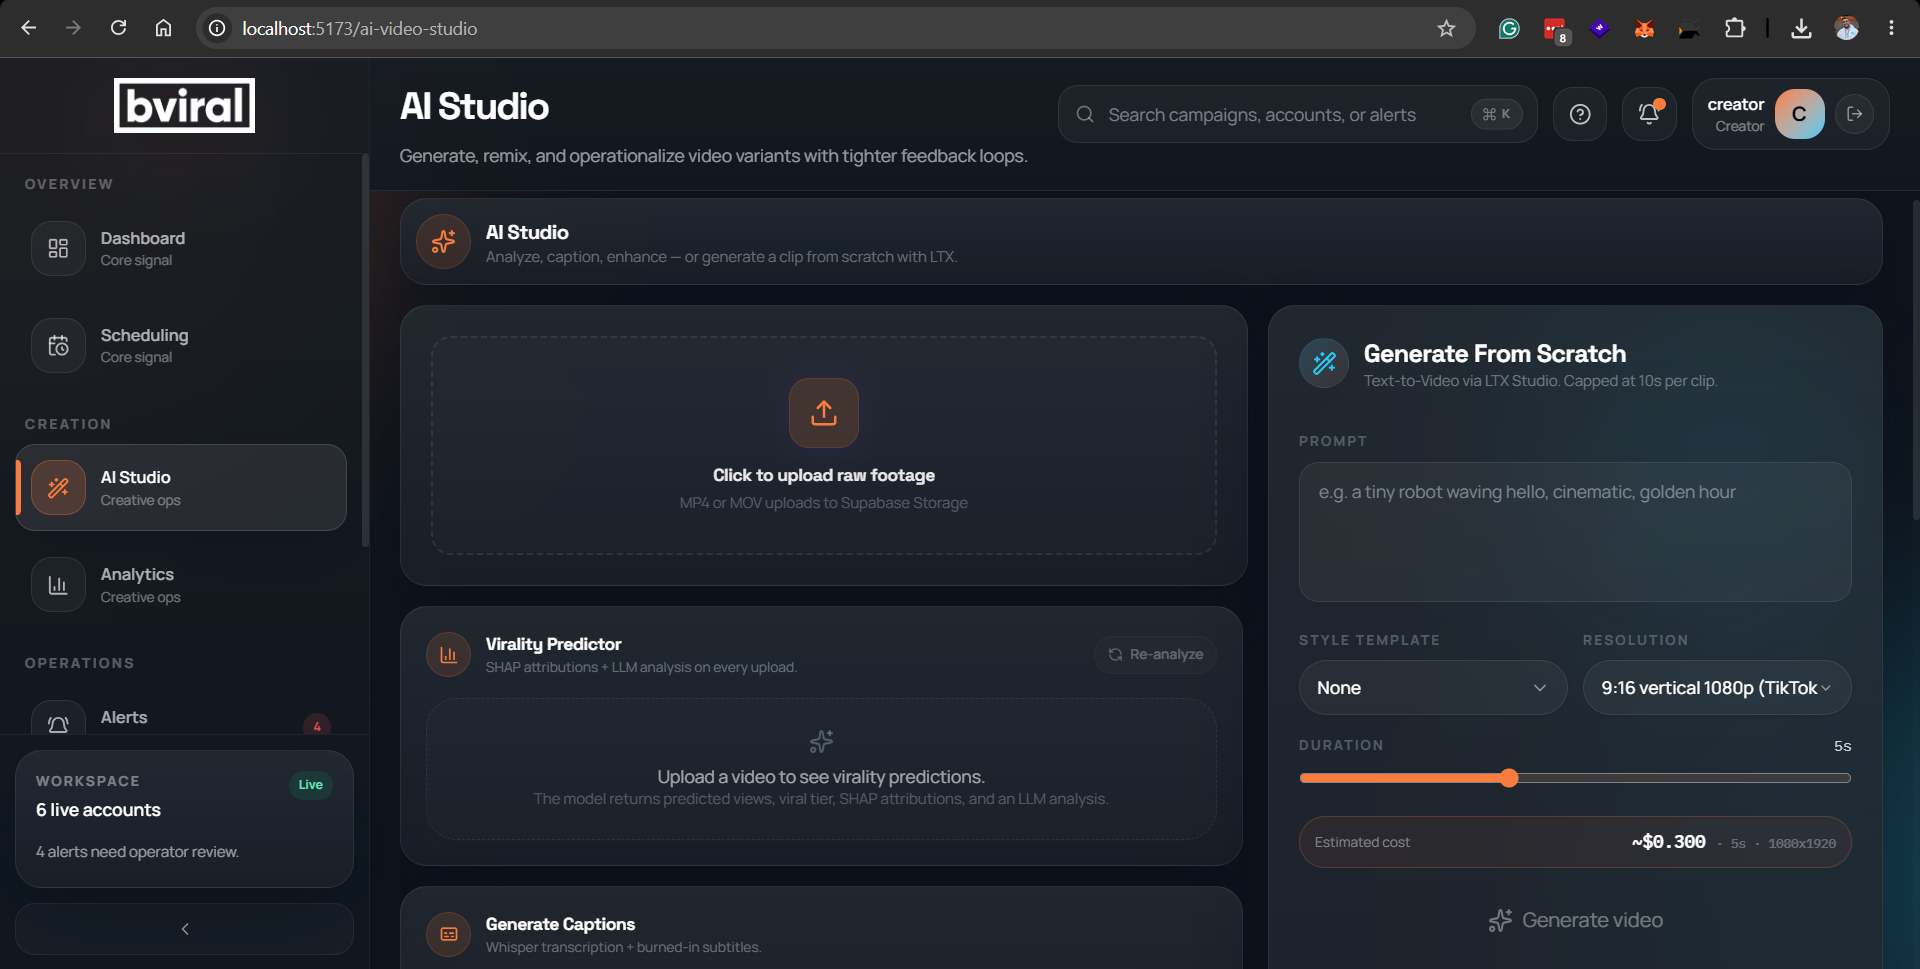
\includegraphics[width=\textwidth]{screens/aistudio.png}
    \caption{Interface: AI Video Studio}
    \label{fig:ui-ai-studio}
\end{figure}

\subsection{Alert Management}

The alerts page displays system notifications in a filterable table. Each alert shows its type (error, copyright, success), associated platform, message, and resolution status. Users can mark alerts as resolved or filter by type and status.

\begin{figure}[H]
    \centering
    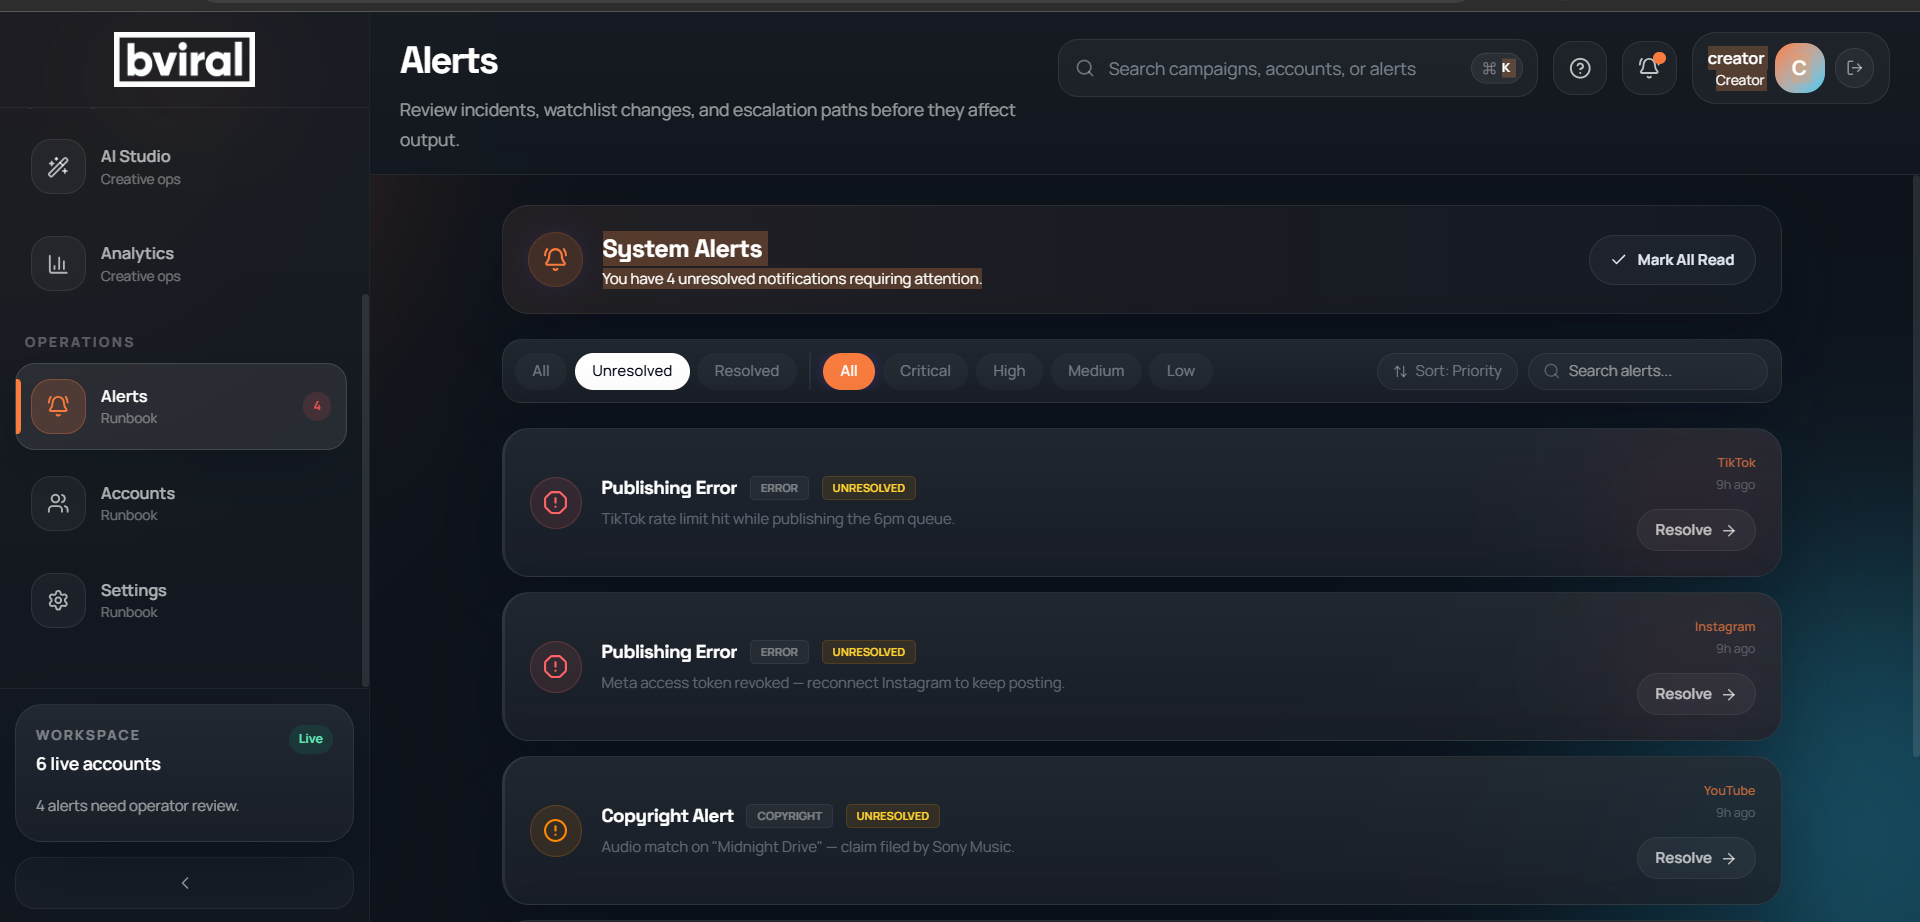
\includegraphics[width=\textwidth]{screens/alerts.png}
    \caption{Interface: Alert management}
    \label{fig:ui-alerts}
\end{figure}

\subsection{Settings}

The settings page allows users to configure their profile, notification preferences, API keys, and system options.

\begin{figure}[H]
    \centering
    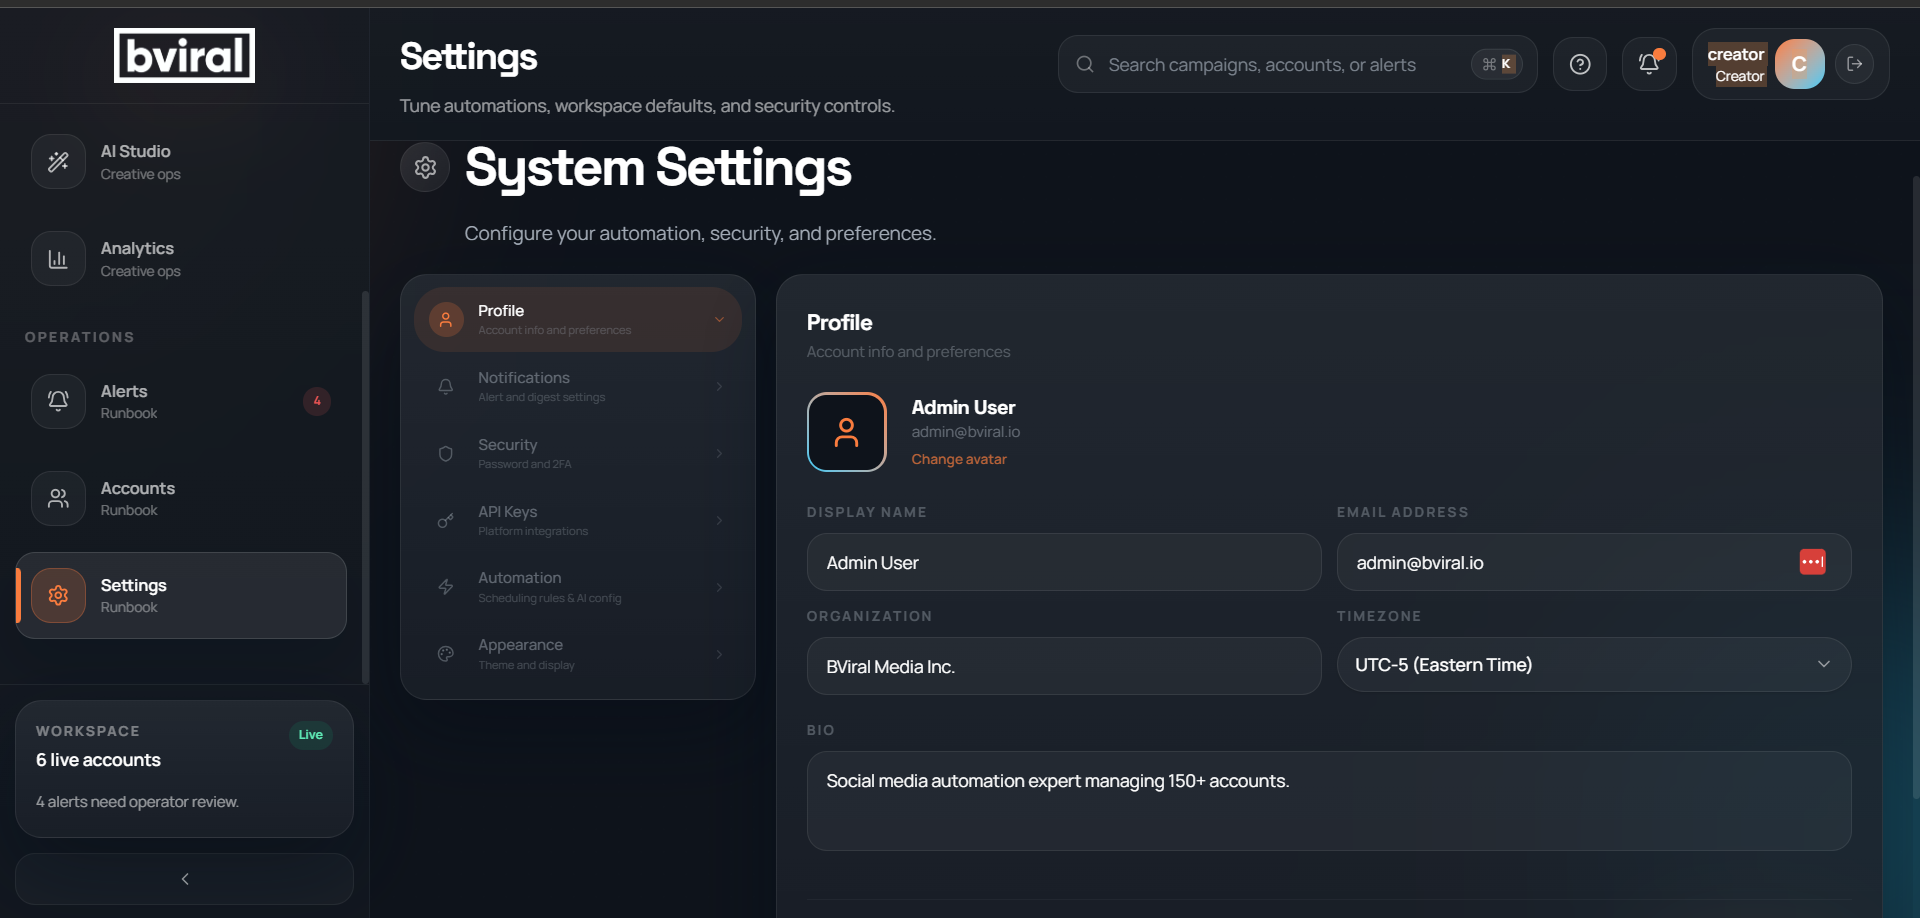
\includegraphics[width=\textwidth]{screens/settings.png}
    \caption{Interface: System settings}
    \label{fig:ui-settings}
\end{figure}

\subsection{Admin Interfaces}

In addition to the creator-facing screens, the dashboard exposes a dedicated admin section accessible only to users with the \texttt{admin} role. Each admin route is guarded both client-side (by the \texttt{AdminOnly} React component) and server-side (by the Fastify \texttt{requireRole("admin")} hook), so a malicious request that bypasses the UI is still rejected at the API layer.

\begin{itemize}
    \item \textbf{Creators:} the administrator can invite, edit, suspend, or remove content creators. A suspended creator can no longer authenticate (the API enforces \texttt{403 Suspended} on every authenticated route except those with the admin role).
    \item \textbf{All Posts:} cross-tenant table of every scheduled or published post in the system, with bulk soft-delete actions.
    \item \textbf{All Videos:} every uploaded video with its owner, derived posts, and processing status.
    \item \textbf{Global Analytics:} aggregated KPIs across all creators with filters, time ranges, and a CSV export.
    \item \textbf{Trash:} posts removed by an admin enter a soft-delete state (column \texttt{deletedAt} populated). The Trash page lets the administrator restore them within the retention window or purge them permanently.
    \item \textbf{Audit Log:} immutable read-only view of the \texttt{admin\_audit\_log} table. Each row exposes the admin, the action, the affected entity, and the JSON payload.
    \item \textbf{System Health:} queue depth and failed-job inspection for the four BullMQ queues, with a one-click retry endpoint.
\end{itemize}

% ══════════════════════════════════════════════════════════════
\section{Security Architecture}
% ══════════════════════════════════════════════════════════════

Security is treated as a cross-cutting concern of the platform rather than a single feature. The design relies on three layered defences: a verified JWT-based authentication, database-level Row-Level Security, and at-rest encryption of every OAuth credential.

\subsection{Supabase JWT Authentication and Role Resolution}

The dashboard performs sign-in against Supabase Auth and stores the returned JWT in the browser session. Each request to the API includes this token in the \texttt{Authorization: Bearer ...} header. The \texttt{50-auth} plugin verifies the token by calling \texttt{<SUPABASE\_URL>/auth/v1/user}, then resolves an internal role using the following priority:

\begin{enumerate}
    \item Explicit claim in the token's \texttt{app\_metadata} (\texttt{app\_role}, \texttt{role}, \texttt{user\_role}, or \texttt{team\_role}) equal to \texttt{admin}.
    \item Otherwise, the \texttt{role} column of the local \texttt{users} table.
    \item Otherwise, the default role \texttt{content\_creator}.
\end{enumerate}

If the resolved user carries a non-null \texttt{suspendedAt} and is not an admin, the request is rejected with \texttt{403 Forbidden}. For local development only, a \texttt{ADMIN\_TOKEN} environment variable enables an automatic admin user attachment to streamline the developer experience; this shortcut is explicitly disabled when \texttt{NODE\_ENV=production}.

\subsection{Row-Level Security (RLS)}

Every business table (\texttt{users}, \texttt{accounts}, \texttt{videos}, \texttt{posts}, \texttt{analytics}, \texttt{alerts}, \texttt{admin\_audit\_log}) has RLS enabled at the PostgreSQL level, with Drizzle-generated \texttt{pgPolicy} declarations. Two families of policies coexist:

\begin{itemize}
    \item \texttt{<table>\_select\_own / insert\_own / update\_own / delete\_own}: a user can only see or modify rows they own (resolved via \texttt{auth.uid()}).
    \item \texttt{admins\_full\_access\_<table>}: a JWT with the \texttt{app\_role = admin} claim is granted full access.
\end{itemize}

This provides defence-in-depth: even if the API layer were compromised or a query forgot a \texttt{WHERE userId = ...} filter, PostgreSQL itself would still refuse to return rows that do not belong to the authenticated user.

\subsection{OAuth Token Encryption at Rest (AES-256-GCM)}

OAuth access and refresh tokens stored in the \texttt{accounts} table are encrypted before persistence using AES-256-GCM, implemented in \texttt{lib/token-encryption.ts}. The storage format is versioned:

\begin{center}
\texttt{enc:v1:<base64url(iv)>:<base64url(authTag)>:<base64url(ciphertext)>}
\end{center}

The encryption key is loaded from the \texttt{TOKEN\_ENCRYPTION\_KEY} environment variable (base64, hex, or a passphrase derived via SHA-256). In production, a missing key causes the API to fail fast at startup. In development, the code falls back to a stable derived key and emits a one-time warning. Legacy plaintext tokens are detected via the absence of the \texttt{enc:v1:} prefix and silently re-encrypted on the next write.

\subsection{TikTok PKCE and Multi-Provider OAuth}

The platform integrates with three OAuth providers (YouTube/Google, TikTok, and Meta for Facebook \& Instagram). TikTok additionally requires PKCE (Proof Key for Code Exchange) and refuses \texttt{localhost} redirect URIs. The implementation keeps the per-attempt PKCE verifier in API memory, and in local development the dashboard is tunneled through \texttt{ngrok} so TikTok accepts the HTTPS redirect URL. Each provider has its own environment configuration; missing credentials return a clean \texttt{503 Service Unavailable} instead of crashing the server.

\subsection{Log Redaction and Sensitive Data Handling}

In production, the Pino logger is configured with a redact list covering \texttt{authorization}, \texttt{cookie}, \texttt{x-admin-token}, \texttt{body.password}, \texttt{*.password}, \texttt{*.secret}, and \texttt{*.token}. This prevents accidental leakage of bearer tokens or user credentials through log aggregation pipelines.

\subsection{Admin Audit Trail}

Every administrative write goes through a single helper, \texttt{writeAudit()}, which inserts a row into the \texttt{admin\_audit\_log} table with the admin id, the action name (e.g.\ \texttt{system.retry\_job}, \texttt{creator.suspend}, \texttt{post.soft\_delete}), the target type, the target id, and a JSON payload describing the operation. The Audit Log admin page is a thin read-only view over this table; the table is indexed on \texttt{(adminId, createdAt)} and \texttt{(targetType, targetId)} for fast forensic lookups.

% ══════════════════════════════════════════════════════════════
\section{Asynchronous Processing and Job Queues}
% ══════════════════════════════════════════════════════════════

Long-running and time-deferred work is delegated to BullMQ workers backed by Redis, keeping the HTTP request path responsive and allowing horizontal scaling of the background fleet.

\subsection{Queue Topology}

Four distinct queues are declared:

\begin{itemize}
    \item \textbf{\texttt{post-publishing}} --- delayed jobs created at the scheduled publication time of each post. Consumed by \texttt{workers/posts.worker.ts}.
    \item \textbf{\texttt{video-processing}} --- video enhancement, super-resolution, and re-encoding jobs. Consumed by \texttt{workers/videos.worker.ts}.
    \item \textbf{\texttt{analytics-refresh}} --- a repeatable cron-style job (\texttt{analyticsRefreshCronPattern}) that pulls fresh metrics from each platform every six hours. Consumed by \texttt{workers/analytics.worker.ts}.
    \item \textbf{\texttt{ai-processing}} --- caption generation, virality prediction, and LTX text-to-video jobs. Consumed by \texttt{workers/ai.worker.ts}.
\end{itemize}

\subsection{Self-Healing on Boot}

When the publishing worker starts, it scans the database for posts whose status is still \texttt{scheduled} and re-enqueues them, including posts that became overdue while the worker was off. This makes the system tolerant to worker restarts, deployments, and short outages without manual intervention.

\subsection{Operational Visibility and Retry}

The \texttt{queuesAdmin} decorator exposed by the queues plugin provides three operations consumed by the System Health admin page:

\begin{itemize}
    \item \texttt{getStats()} --- counts of waiting, active, completed, failed, delayed, and paused jobs per queue.
    \item \texttt{getFailedJobs(queueName, limit)} --- inspection of the most recent failed jobs (name, failure reason, attempts, timestamps).
    \item \texttt{retryJob(queueName, jobId)} --- one-click re-enqueue of a specific failed job, with a corresponding audit log entry.
\end{itemize}

% ══════════════════════════════════════════════════════════════
\section{API Specification and Type-Safe Code Generation}
% ══════════════════════════════════════════════════════════════

A recurring source of bugs in client--server applications is drift between the contract documented by the backend and the assumptions made by the frontend. To eliminate this drift, the BViral codebase treats the OpenAPI 3.1 specification (\texttt{lib/api-spec/openapi.yaml}) as the single source of truth. From this file, two libraries are auto-generated:

\begin{itemize}
    \item \texttt{lib/api-zod} --- runtime Zod validation schemas, consumed by the Fastify route handlers and the workers for inbound payload validation.
    \item \texttt{lib/api-client-react} --- TanStack Query hooks (\texttt{useListPosts}, \texttt{useCreatePost}, \texttt{useListAccounts}, etc.) with full TypeScript types, consumed directly by the dashboard.
\end{itemize}

Any change to the OpenAPI specification regenerates both libraries; the TypeScript compiler then surfaces every call site that needs to be updated. This guarantees compile-time and runtime alignment between the API and its only first-party client.

% ══════════════════════════════════════════════════════════════
\section{Multi-Platform Publishing Abstraction}
% ══════════════════════════════════════════════════════════════

The diversity of social-media APIs (YouTube Data API, TikTok Open API, Meta Graph API) is hidden behind a single \texttt{platform-publisher.service}. Each provider has its own service (\texttt{youtube.service}, \texttt{tiktok.service}, \texttt{meta.service}) implementing a uniform \texttt{publish(post, account, video)} interface. The publishing worker dispatches a job to the correct provider based on the \texttt{platform} column of the post. New providers (e.g.\ Snapchat) can be added with no change to the worker or to the API contract --- the database enum already includes the platform value.

% ══════════════════════════════════════════════════════════════
\section{AI Component Design}
% ══════════════════════════════════════════════════════════════

The artificial intelligence ecosystem within BViral Control Center is structured around three independent but complementary pillars: the Pre-Posting Predictive Agent, the Auto-Captioning Engine, and the Video Quality Enhancement Engine.

\begin{figure}[H]
    \centering
    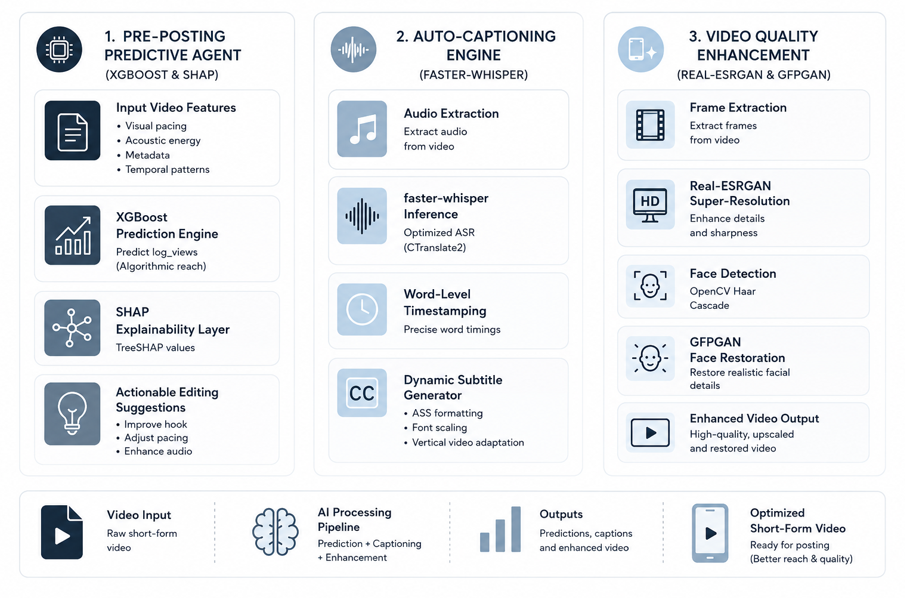
\includegraphics[width=0.8\textwidth]{images/aidesign.png}
    \caption{AI component design of BViral Control Center}
    \label{fig:ai_design}
\end{figure}

\subsection{Algorithm Selection and Justification}

Each pillar utilizes specific algorithms chosen for their performance, hardware efficiency, and suitability for the task:

\begin{itemize}
    \item \textbf{Pillar 1: Pre-Posting Predictive Agent (XGBoost \& SHAP):} 
    To predict a video's algorithmic reach (\texttt{log\_views}), we selected \textbf{XGBoost (eXtreme Gradient Boosting)}. Unlike Deep Neural Networks which are prone to overfitting on tabular data of this size ($\sim$1,100 rows), XGBoost excels at capturing complex, non-linear interactions between multimodal features (e.g., visual pacing vs. acoustic energy). Crucially, XGBoost integrates flawlessly with \textbf{TreeSHAP} (SHapley Additive exPlanations), allowing the system to reverse-engineer the prediction and provide explainable, actionable editing advice to the creator.
    
    \item \textbf{Pillar 2: Auto-Captioning Engine (\texttt{faster-whisper}):}
    Standard OpenAI Whisper models are highly accurate but computationally heavy. We justified the use of \texttt{faster-whisper},a reimplementation that drastically reduces VRAM usage while running up to 4 times faster. It extracts precise word-level timestamps, which are then passed to a custom font-scaling algorithm to dynamically generate \texttt{.ass} subtitle scripts formatted specifically for short-form vertical screens.
    
    \item \textbf{Pillar 3: Video Quality Enhancement (Real-ESRGAN \& GFPGAN):}
    For super-resolution, we selected \textbf{Real-ESRGAN}, a Generative Adversarial Network optimized for restoring real-world degraded videos by hallucinating missing high-frequency details. Because standard GANs often distort human faces, we integrated \textbf{GFPGAN} as a secondary pass specifically triggered by OpenCV Haar Cascade face detection. GFPGAN leverages generative facial priors to reconstruct realistic eyes, teeth, and skin textures.
\end{itemize}



% ══════════════════════════════════════════════════════════════
\section*{Conclusion}
% ══════════════════════════════════════════════════════════════

In this chapter, we presented the technical architecture of BViral Control Center, justified our technology choices, and showcased the implemented interfaces. The monorepo workspace architecture provides a clean separation between the React dashboard and the Fastify API server. Furthermore, the integration of a highly complex, three-pillar AI ecosystem—featuring an XGBoost Predictive Agent, a Whisper-driven Auto-Captioning engine, and a Real-ESRGAN/GFPGAN enhancement pipeline distinguishes our solution from standard social media management tools by offering creator-focused algorithmic diagnostics and production-grade video processing.

\phantomsection
\addcontentsline{toc}{section}{Conclusion}


